\chapter{A rede social Portal de Vagas}
\label{redeSocialPortal}

Este capitulo descreve as funcionalidades presentes e ausentes no prótotipo de rede social Portal de Vagas. Primeiramente, é apresentado o funcionamento e todas interações possíveis em cada página do sistema. Em seguida, são listadas as limitações que a versão final do protótipo possui e, posteriormente, sugeridas melhorias como guia para trabalhos futuros. Por fim, é apresentado uma tabela comparativa, de maneira similar à seção \ref{trabRelAnalise}; porém, com o acréscimo do Portal de Vagas ao compartivo.

\section{Funcionamento}
\label{PDVFuncionamento}

Nesta seção será apresentado o funcionamento da rede social Portal de Vagas, explicando as funcionalidades e possibilidades de interação entre os usuários e as vagas ofertadas em todas as páginas do sistema: \textit{Login}, Inicial, Perfil de usuário, Vagas disponíveis e favoritas, Vaga específica, Configurações da conta de usuário. Além disso, será detalhado como é a realização de consultas comuns e avançadas sobre vagas, usuários e sistema de inscrição em vagas.

\subsection{Página de \textit{Login}}
\label{PDVFunLogin}

A rede social só pode ser utilizada através da autenticação de usuários cadastrados no sistema. Dessa forma, caso algum usuário não autenticado tente acessar uma página interna e válida do sistema escrevendo diretamente sua URL no navegador, ele será redirecionando para a tela de \textit{login} automaticamente. Em contrapartida, caso o usuario já esteja autenticado e tente acessar a página de \textit{Login} é redirecionado então para a página Inicial.

A página apresenta um visual simples e objetivo, com o logotipo do INF e abaixo um formulário contendo um campo de nome de usuário ou \textit{e-mail} e um para a senha. Contudo, como é mencionado na seção \ref{redeLimitacao}, por ser tratar de um protótipo, todos os usuários foram criados em um banco de dados exclusivo da aplicação. Dessa forma, não há de fato uma integração com o banco de dados de usuários da UFRGS, ou seja, não existe possibilidade, nesta implementação, de um usuário se autenticar com as mesmas credenciais em ambos os sistemas sem a criação prévia deste registro no banco do protótipo apresentado. 

Ainda, no final do formulário, existe um link para o usuário recuperar sua senha em caso de esquecimento. Como essa funcionalidade não seria necessária no protótipo, o link apenas redireciona o usuário para a página de recuperação de senha\footnote{\url{https://www.inf.ufrgs.br/portal/login.php\#resetpasswd} Acesso em novembro de 2018} na área de Administração de Rede do site do INF.

A Figura \ref{telaLoginImg} apresenta a página de \textit{Login} com os campos de usuário e senha disponíveis para preenchimento. Só após a correta autenticação, as demais páginas da rede social ficam acessíveis.

\begin{figure}[h]
    \caption{Tela de \textit{login} do Portal de Vagas.}
       	\begin{center}
            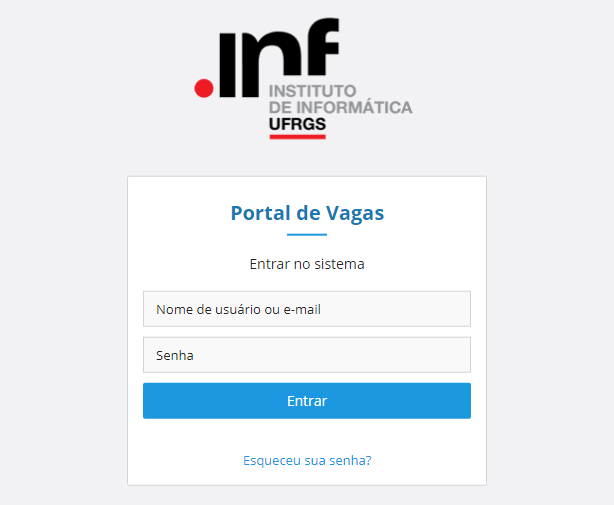
\includegraphics[width=0.85\textwidth]{figuras/tela_login.png}
        \end{center}
    \label{telaLoginImg}
    \legend{Fonte: Autor}
\end{figure}

\subsection{Página inicial}
\label{PDVFunFeed}

A página inicial do Portal de Vagas, acessada após o usuário se autenticar no sistema é composta por três seções: painel com dados resumidos do usuário, lista de postagens das pessoas seguidas na conta e painel de sugestões para seguir outros usuários e analisar vagas ofertadas, de forma a estimular o usuário a explorar a rede social. A Figura \ref{telaHome} exibe a Página inicial do sistema com suas três seções.

O painel com os dados resumidos apresenta a foto de perfil do usuário; seguido por seu nome; sua profissão, escolaridade ou local onde mora de acordo com os dados preenchidos; número de seguidores e desde quando realizou seu primeiro\textit{login} no sistema.

A lista de postagens começa com um campo de texto onde é possível o usuário realizar sua própria postagem que será exibida no \textit{feed} de seus seguidores. Da mesma forma, abaixo deste espaço, são apresentadas todas as postagens das pessoas que são seguidas pelo usuário. Nestas postagens, é possível curti-las e comentá-las também. Contudo, como a funcionalidade proposta seria uma alternativa aos e-mails de graduação, após comentar numa postagem, não é permitida a edição nem remoção deste, simulando assim um comportamento de serviço de \textit{webmail}.

Por fim, o painel de sugestões lista cinco usuários e vagas como sugestão para interação na rede social. Para as pessoas sugeridas, são ocultadas da lista as que o usuário já segue ou bloqueou. Além disso, ambas as listas são ordenadas pelo critério de relevância, isto é, as que possuem mais recomendações são apresentadas primeiro.

\begin{figure}[ht]
    \caption{Página inicial da rede social.}
       	\begin{center}
            \includegraphics[width=1\textwidth]{figuras/arquitetura-centralizada-dados.png}
        \end{center}
    \label{telaHome}
    \legend{Fonte: Autor}
\end{figure}

\subsection{Página de perfil de usuário}
\label{PDVFunProfile}

A Página de perfil de usuário, semelhante a Página inicial, exibe informações sobre a pessoa que estamos acessando o perfil. Ela também é dividida em três seções principais, sendo elas: informações básicas de perfil, recomendações de outros usuários e um painel com sugestões de outras pessoas para interagir.

A seção de informações básicas pode ser editável contanto que o usuário autenticado esteja visitando o seu próprio perfil. Caso contrário, a página é apenas para leitura. Os dados são exibidos de forma completa e segmentados nos seguintes blocos: informações gerais, experiências profissionais, educação, habilidades profissionais e idiomas. Em informações gerais são apresentados um resumo dos dados mais importantes e recentes da pessoa como trabalho e educação mais recentes, localização, número de seguidores, desde quando está ativo no sistema e uma breve autodescrição. As experiências profissionais e educacionais são uma lista de dados ordenados da mais recente à mais antiga. Contudo, o usuário pode selecionar uma experiência para deixar destacada e ser a primeira a ser exibida (independente da ordenação inicial).Habilidades profissionais são uma lista de \textit{tags} acompanhadas do nível de experiência e tempo que possui tal conhecimento, apresentando uma lista bem sucinta das principais qualificações da pessoa. Por fim, de forma similar, há o bloco de idiomas que o usuário pode indicar e quantificar as línguas que ele possui fluência.

A seção de recomendações é um espaço para outras pessoas interagirem com o perfil do usuário visitado. Ali é possível recomendá-lo positivamente na rede social, qualificando-o individualmente e estimulando coletivamente as interações entre usuários. Além disso, é interessante considerar o cenário onde um professor esteja em dúvida sobre qual candidato aceitar em uma vaga ofertada: através das recomendações ele pode ter uma ideia mais concreta sobre a pessoa que estaria disposto a selecionar como seu bolsista, por exemplo. Ainda sobre a seção, um usuário só pode recomendar outros uma única vez e, obviamente, não pode recomendar a si mesmo.

Por último, o painel de pessoas sugeridas para o usuário seguir segue os mesmos critérios de ordenação da Página inicial. A diferença é que o número de sugestões é maior -dez pessoas- e não são sugeridas vagas na Página de perfil. A Figura \ref{telaUserProfile} apresenta a Página de perfil de usuário com todas as seções citadas.

\begin{figure}[ht]
    \caption{Página de perfil de usuário.}
       	\begin{center}
            \includegraphics[width=1\textwidth]{figuras/arquitetura-centralizada-dados.png}
        \end{center}
    \label{telaUserProfile}
    \legend{Fonte: Autor}
\end{figure}

\subsection{Página de vagas disponíveis}
\label{PDVFunVagas}

A Página de vagas fornece ao usuário uma lista de todas as vagas disponíveis no sistema, sejam elas bolsa de monitoria, iniciação científica, estágio, ou até mesmo de efetivo. Uma das propostas do Portal de Vagas é uma releitura da página de vagas ofertadas no Mural de Bolsas.A estrutura da página é composta por duas seções principais: a área de filtros de pesquisa e a lista de vagas disponíveis.

A área de filtros foi expandida em relação ao Mural de Bolsas. Agora é possível filtrar por localidade e também incorporar as funcionalidades integradas de vagas que exigem currículos e/ou histórico escolar. Além disso, é possível selecionar o método de ordenação: mais relevantes, melhores avaliados, mais recentes e mais antigos. No MB a listagem era ordenada pelas vagas mais recentes primeiro. Por padrão, a lista de filtros é oculta e, se o usuário sentir necessidade, pode expandi-la e aplicar os filtros desejados. A Figura \ref{telaFiltros} exibe a seção em formato expandido com todos os campos possíveis.

\begin{figure}[ht]
    \caption{Lista de filtros expandidos.}
       	\begin{center}
            \includegraphics[width=1\textwidth]{figuras/arquitetura-centralizada-dados.png}
        \end{center}
    \label{telaFiltros}
    \legend{Fonte: Autor}
\end{figure}

A lista de vagas é apresentada em uma visão de \textit{cards}, onde cada cartão apresenta as conjunto de informações compacto com "título", "localização", "áreas de atuação", "resumo", "remuneração" e "carga horária". Além disso, possui um botão para salvar a vaga na lista de favoritos do usuário; o botão "Candidatar-se" para se inscrever numa vaga disponível (ver seção \ref{PDVFunInscricoes}) e o botão "Ver mais" que abre a página da vaga selecionada com todas suas informações e recomendações. A Figura \ref{telaVagasLista} apresenta a visualização de vagas disponíveis.

\begin{figure}[ht]
    \caption{Lista de vagas disponíveis em formato de \textit{card}.}
       	\begin{center}
            \includegraphics[width=1\textwidth]{figuras/arquitetura-centralizada-dados.png}
        \end{center}
    \label{telaVagasLista}
    \legend{Fonte: Autor}
\end{figure}

\subsection{Página de vaga específica}
\label{PDVFunVaga}

A Página de vaga específica é uma versão completa dos \textit{cards} apresentados na página de Lista de vagas. Essa página apresenta três seções: a área de informação de vaga, o painel com lista de vagas relacionadas e a área de recomendações. Se o usuário que acessa a página é o próprio autor da vaga, existe ainda uma quarta seção: a de candidatos inscritos. A Figura \ref{telaVagaCompleta} exibe a página da Vaga de maneira completa com todas as seções disponíveis.

A área de informação da vaga, em ordem de exibição, contempla os seguintes dados: "título da vaga", "localização", "áreas de interesse", "autor da vaga", "descrição completa", "modalidade", "tipo de vaga", "experiência exigida", "carga horária", "turnos", "data de início", "duração", "exigência de currículo", "exigência de histórico escolar", "benefício PRAE". Alguns dados podem ser omitidos caso o autor da vaga opte por deixar alguma informação opcional em branco. Ao final, existe um botão de "Candidatar-se" também caso o usuário não tenha se inscrito na vaga ainda.

A seção de recomendações é uma lista com todas as recomendações enviadas por usuários que decidiram avaliar positivamente a vaga ofertada. Cada recomendação contém dados básicos do autor e o texto explicando o motivo da avaliação. Os usuários podem recomendar cada vaga uma única vez.

No canto superior direito, existe também um painel com uma lista de vagas semelhantes que possam interessar o usuário, facilitando assim o fluxo de navegação. O critério de ordenação é a relevância da vaga, isto é, as que possuem mais recomendações e mais favoritadas, vêm primeiro.

Por fim, para a situação em que o usuário autenticado é também o autor da vaga...

\begin{figure}[ht]
    \caption{Página de vaga com todas informações disponíveis.}
       	\begin{center}
            \includegraphics[width=1\textwidth]{figuras/arquitetura-centralizada-dados.png}
        \end{center}
    \label{telaVagaCompleta}
    \legend{Fonte: Autor}
\end{figure}

\subsection{Página de Favoritos}
\label{PDVFunFavoritos}

A Página de favoritos é apenas uma comodidade oferecida pelo sistema. Nela se encontram todas as vagas que estão favoritadas pelo usuário. Dessa forma, a página já oferece uma lista de vagas que atendem a esse critério inicial. Além disso, os filtros tradicionais presentes na página de Vagas também estão disponíveis para uso e posterior refinamento de pesquisa. A Figura \ref{telaVagaFav} apresenta todas as vagas favoritas pelo usuário: repare que o ícone de estrela fica destacado na cor azul.

\begin{figure}[ht]
    \caption{Página de vagas favoritas do usuário.}
       	\begin{center}
            \includegraphics[width=1\textwidth]{figuras/arquitetura-centralizada-dados.png}
        \end{center}
    \label{telaVagaFav}
    \legend{Fonte: Autor}
\end{figure}

\subsection{Página de inscrições}
\label{PDVFunInscricoes}

A Página de inscrições apresenta a lista de inscrições dos usuários em vagas ofertadas pelo sistema. Ela apresenta três seções importantes: a área de filtro, a lista de inscrições e o painel de sugestões. duas exibições diferentes que levam em conta o papel do usuário no sistema. Se ele for um aluno, a página apresentará uma lista com todas as vagas que este se inscreveu. Se for professor, então a lista será de todos os alunos que se inscreveram nas vagas criadas por ele.

Em ambos os papéis, a área de filtros apresenta o mesmo comportamento: ela fornece um formulário com 3 \textit{checkboxes} que descrevem a situação em que se encontra a instrição. São elas: "em avaliação" (ou "avaliação pendente" se for professor), "aprovado" e "reprovado". Por padrão, a opção que vem marcada filtra os resultados para exibir apenas as inscrições em andamento, pois é a informação de maior interesse dos autores e candidatos da vaga.

O painel de sugestões mantém o mesmo princípio das páginas anteriores e exibe uma lista com as vagas ofertadas na rede social ordenadas da maior para a menor relevância.

A principal diferença das seções ocorre na listagem. Quando um aluno se candidata a uma vaga, o professor recebe um e-mail notificando-o sobre uma nova inscrição. Nesse momento, o \textit{status} da inscrição é marcado como "em avaliação". Quando o professor avalia a inscrição e opta por aprovar ou reprovar a candidatura, o aluno também é notificado por e-mail. As diferenças entre as telas para os dois usuários estão representadas nas Figuras \ref{telaInscrAluno} e \ref{telaInscrProf}.

\begin{figure}[h]
    \caption{Tela de inscrições para alunos.}
       	\begin{center}
            \includegraphics[width=0.75\textwidth]{figuras/arquitetura-centralizada-dados.png}
        \end{center}
    \label{telaInscrAluno}
    \legend{Fonte: Autor}
\end{figure}

\begin{figure}[h]
    \caption{Tela de inscrições para professores.}
       	\begin{center}
            \includegraphics[width=0.75\textwidth]{figuras/arquitetura-centralizada-dados.png}
        \end{center}
    \label{telaInscrProf}
    \legend{Fonte: Autor}
\end{figure}

\subsection{Página de pesquisa}
\label{PDVFunPesquisa}

Sempre que o usuário sentir necessidade de procurar por usuários ou vagas de um modo mais genérico, ele pode realizar a consulta digitando um termo de interesse no campo de pesquisa no cabeçalho de todas as páginas. Assim, ele será direcionado para a página de Pesquisa que exibe todos resultados encontrados tanto nas vagas quanto em usuários cadastrados no sistema. A Figura \ref{PDVPesquisaTela} mostra a tela de resultados encontrados na págia de Pesquisa.

A página ainda fornece ao usuário a possibilidade filtrar os resultados por "pessoas" ou "vagas". Além disso, no canto direito, existe um painel listando os 10 termos mais recentes e pesquisados na rede social, ordenados do maior para o menor.

\begin{figure}[ht]
    \caption{Página de Pesquisa: exemplo de tela com os resultados para a pesquisa pelo termo "lsa". }
       	\begin{center}
            \includegraphics[width=0.68\textwidth]{arquitetura-centralizada-dados.png}
        \end{center}
    \label{PDVPesquisaTela}
    \legend{Fonte: Autor}
\end{figure}

\subsection{Páginas de preferências do usuário}
\label{PDVFunConfiguracoes}

As páginas de preferências são um agregado de opções que a rede social oferece de forma que os usuários possam escolher o comportamento do Portal de Vagas em determinadas ações como: exibição ou não de currículo e histórico escolar, nome de exibição no sistema, \textit{e-mail} para notificações do sistema.

Por padrão, a primeira tela é sempre a de Configurações gerais. Ao lado esquerdo, existe um painel com uma lista para acesso rápido de todas as opções oferecidas ao usuário. Ao lado direito, são exibidos campos do formulário da página em questão. Foi adicionado também um destaque no link de acesso rápido referente à página em questão. Isto é, o \textit{link} fica em negrito, sublinhado e azul.

\subsubsection{Configurações gerais}
\label{PDVFunConfiguracoesGeral}

A tela de Configurações gerais apresenta um formulário com quatro campos. O primeiro é o nome de exibição do usuário no sistema. O campo de \textit{e-mail} serve como complemento aos já fornecidos pelo INF e UFRGS. Neste caso, a ideia é o usuário ter a possibilidade de cadastrar um e-mail em uma plataforma que ele utilize com maior frequência, pois facilitaria o recebimento de notificações enviadas pelo Portal de Vagas. O telefone é um campo não obrigatório e só é exibido para o autor de uma vaga ofertada caso o usuário demonstre interesse por esta. Por fim, há o campo de idioma onde o usuário pode alternar entre as diferentes linguagens ofertadas pela rede social (para o protótipo apenas a lingua portuguesa está disponível). A Figura \ref{telaConfigGeral} apresenta a tela de Configurações gerais.

\begin{figure}[ht]
    \caption{Tela de Configurações gerais.}
       	\begin{center}
            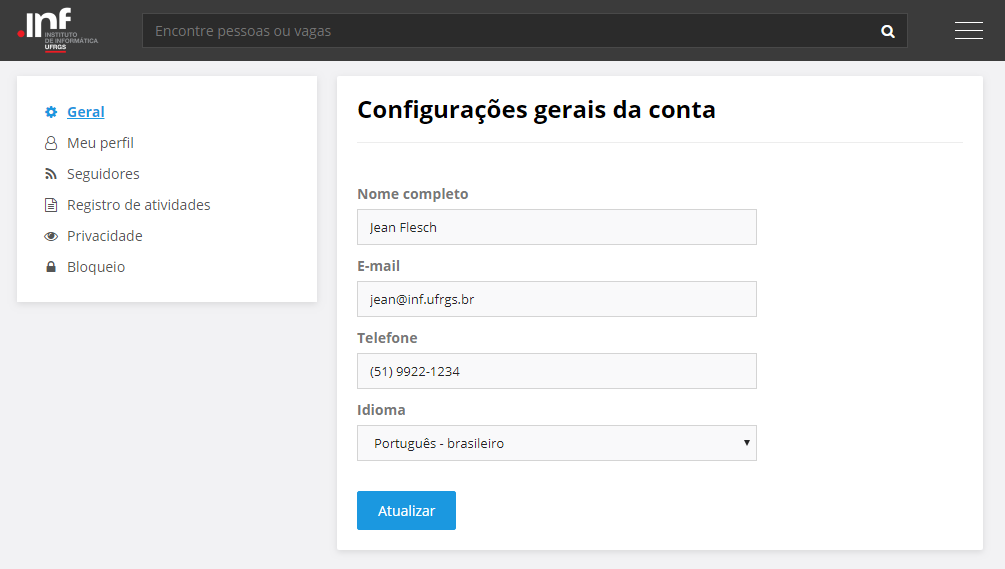
\includegraphics[width=1\textwidth]{figuras/config_01.png}
        \end{center}
    \label{telaConfigGeral}
    \legend{Fonte: Autor}
\end{figure}

\subsubsection{Lista de seguidores}
\label{PDVFunConfiguracoesListaSeguidores}

A página de Lista de seguidores exibe todos os seguidores do usuário, de maneira ordenada, do mais recente ao mais antigo. Existem duas seções na página: a primeira é um parágrafo informativo sobre como as configurações de privacidade afetam na exibição da lista de seguidores para outros usuários do sistema; a segunda é, de fato, a lista de usuários seguidores. Cada registro possui um link direto para o perfil do seguidor. A Figura \ref{telaConfigSeguidores} exibe a página da Lista de seguidores.

\begin{figure}[ht]
    \caption{Tela de seguidores do usuário.}
       	\begin{center}
            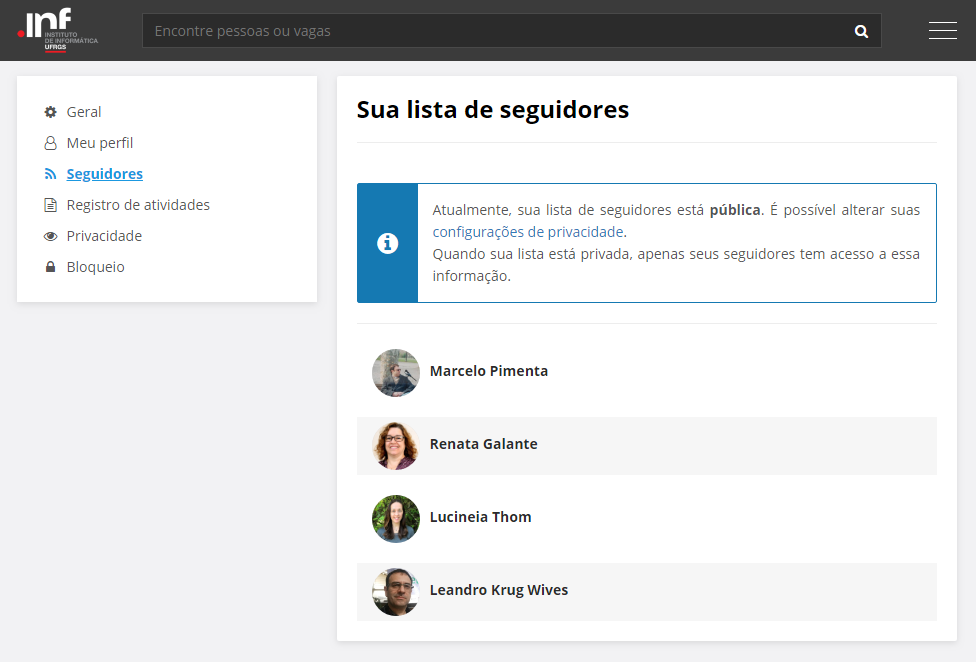
\includegraphics[width=1\textwidth]{figuras/config_05.png}
        \end{center}
    \label{telaConfigSeguidores}
    \legend{Fonte: Autor}
\end{figure}

\subsubsection{Registro de atividades}
\label{PDVFunConfiguracoesLog}

A página de Registro de atividades funciona como um histórico de todas as ações significativas de um usuário no Portal de Vagas. As ações são apresentadas em um formato de linha do tempo onde o mais recente é o primeiro a ser exibido. Cada registro possui texto e ícones personalizadas para diferenciação.

Os seguintes eventos são considerados ações significativas e, consequentemente, exibidos no Registro de atividades:

\begin{itemize}
    \item Realizar primeiro login no sistema;
    \item Atualizar foto de perfil;
    \item Curtir uma postagem;
    \item Comentar em uma postagem;
    \item Favoritar ou desfavoritar uma vaga;
    \item Demonstrar interesse numa vaga;
    \item Recomendar usuário ou vaga
    \item Seguir ou deixar de seguir usuário;
    \item Bloquear ou desbloquear usuário;
    \item Aprovar ou reprovar um candidato numa vaga;
    \item Criar, editar ou deletar vaga;
\end{itemize}

\begin{figure}[h]
    \caption{Tela de Registro de atividades do usuário.}
       	\begin{center}
            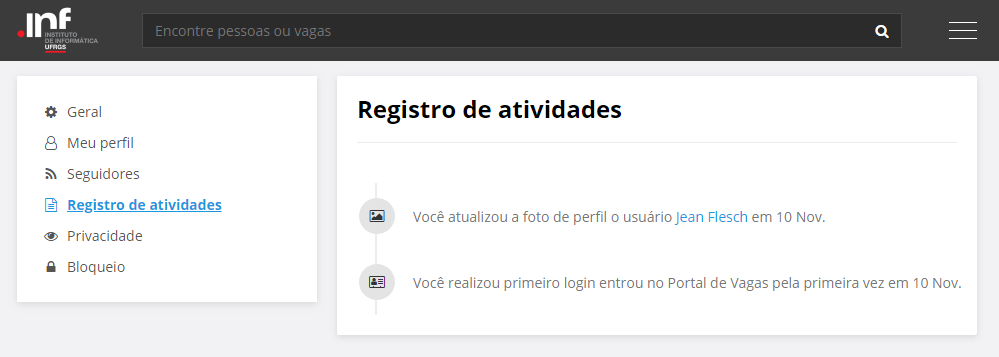
\includegraphics[width=1\textwidth]{figuras/config_03.png}
        \end{center}
    \label{telaConfigLog}
    \legend{Fonte: Autor}
\end{figure}

\subsubsection{Configurações de privacidade}
\label{PDVFunConfiguracoesPrivacidade}

A página de Configurações de privacidade fornece flexibilidade ao usuário para que ele possa controlar o quais informações são visíveis às demais pessoas da rede social. Para este protótipo, foram propostas as seguintes opções de privacidade:

\begin{itemize}
    \item \textbf{Visibilidade das publicações:} todos os usuários têm acesso (público) ou apenas seguidores (privado);
    
    \item \textbf{Histórico escolar:} se o usuário deixar visível, outras pessoas poderão ver os conceitos deste em sua página de perfil. Caso contrário, a informação é oculta. Independentemente da escolha do usuário nesta opção, quando ele se candidata a uma vaga que exige histórico escolar, seus dados são enviados ao autor da vaga.
    
    \item \textbf{Currículo:} o funcionamento é o mesmo que na opção de histórico escolar: o usuário pode ocultar ou não a informação em seu perfil, mas se ele se candidata a uma vaga que exige currículo, a informação é enviada automaticamente ao autor da vaga.
    
    \item \textbf{Visibilidade da lista de seguidores:} todos os usuários têm acesso (público) ou apenas seguidores (privado);
    
    \item \textbf{Visibilidade da lista de seguidos:} todos os usuários têm acesso (público) ou apenas seguidores (privado)
\end{itemize}

\begin{figure}[ht]
    \caption{Tela de Configurações de privacidade.}
       	\begin{center}
            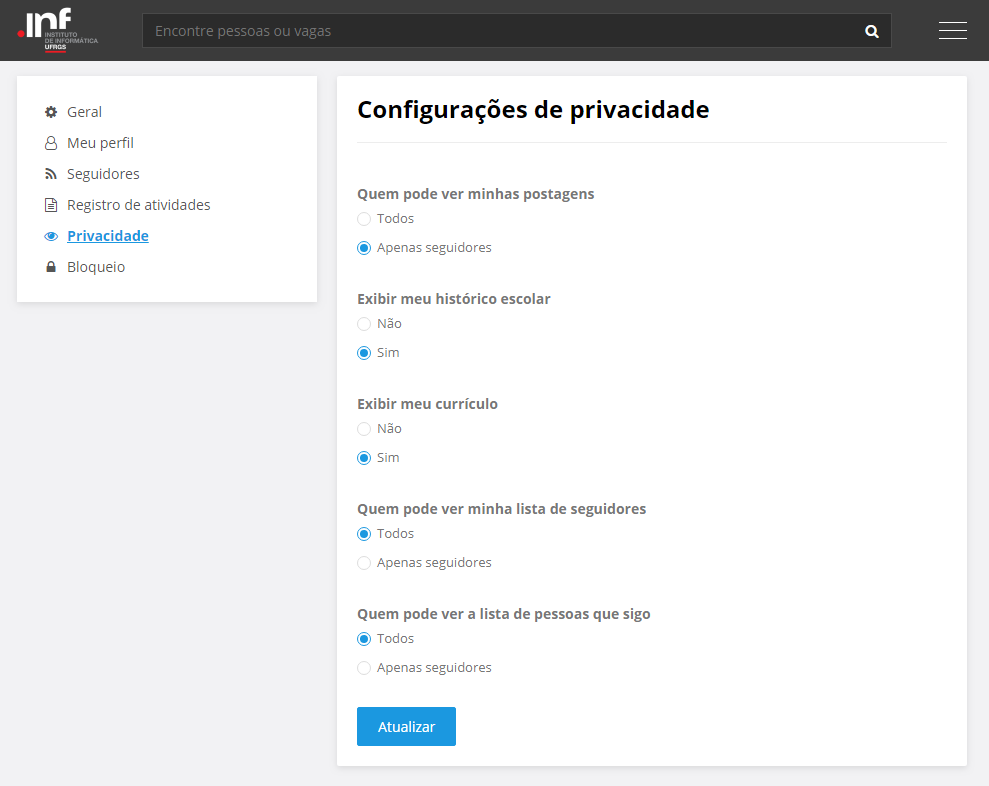
\includegraphics[width=0.68\textwidth]{figuras/config_02.png}
        \end{center}
    \label{telaConfigPrivacidade}
    \legend{Fonte: Autor}
\end{figure}

\subsubsection{Lista de bloqueados}
\label{PDVFunConfiguracoesBloq}

Assim como a Lista de seguidores, a página com a Lista de bloqueados é uma funcionalidade que prioriza uma melhor experiência de usuário. Nesta situação, a página apresenta também duas seções: a primeira informa ao usuário as consequências de adicionar outra pessoa na sua lista de bloqueados; a segunda, é a lista de todos os usuários bloqueados.

As principais consequências de bloquear um usuário são: ele não aparecerá na lista de sugestões de usuários para seguir; as publicações dele ficam ocultas, não é possível comentar em posts criados por ele nem recomendar vagas que ele publicar. Entretanto, o bloqueio não é bidirecional, isto é, ele ainda poderá ter acesso a quaisquer informações compartilhadas publicamente. A Figura \ref{telaConfigBloq} exibe o visual da página de usuários bloqueados.

\begin{figure}[ht]
    \caption{Tela de usuário bloqueados.}
       	\begin{center}
            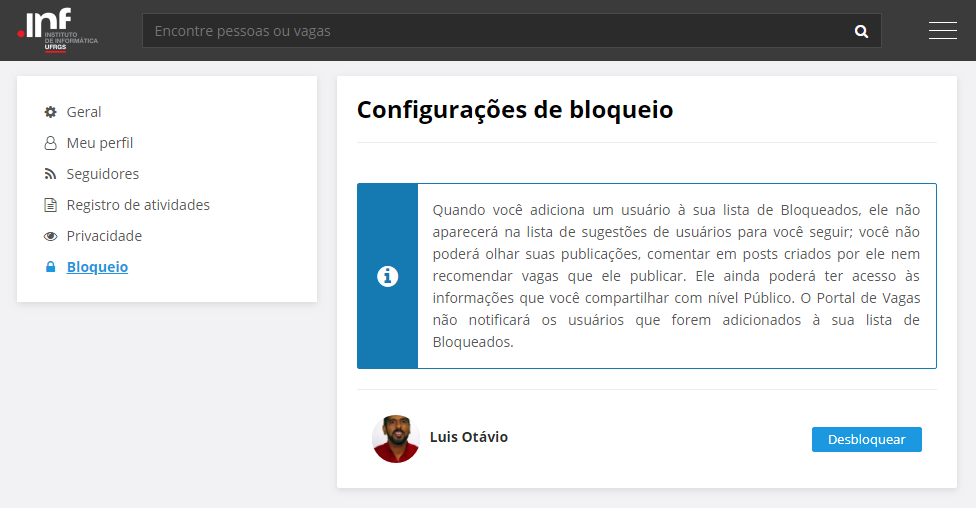
\includegraphics[width=0.95\textwidth]{figuras/config_04.png}
        \end{center}
    \label{telaConfigBloq}
    \legend{Fonte: Autor}
\end{figure}

\section{Limitações e trabalhos futuros}
\label{redeLimitacao}

A rede social Portal de Vagas, por se tratar de um protótipo, possui limitações de sistema. Para tornar possível sua aplicação completa, são necessários alguns passos adicionais. O primeiro e mais importante seria a realização de uma integração real com as demais ferramentas utilizadas pela UFRGS. Por exemplo: a funcionalidade de obter o histórico escolar do aluno e enviar seu currículo automaticamente por e-mail ao responsável pela vaga foi implementada no protótipo com o envio de um arquivo estático em formato \textit{.pdf}. Na versão final, um passo adicional seria realizar uma consulta ao banco de dados utilizado no Portal do Aluno e retornar os valores que lá são apresentados. Além disso, outras ferramentas como o próprio Moodle e o \textit{Webmail} poderiam ser utilizados para aumentar a experiência de usuário. 

O Moodle mantém as informações de turmas que o aluno cursou em sua jornada acadêmica. Dessa forma, o critério de ordenação por relevância em vagas poderia se valer de uma inteligência artificial mais sofisticada e atribuir um peso maior para vagas relacionadas às disciplinas cursadas. Essa estratégia seria bastante útil com cadeiras eletivas, visto que elas abordam assuntos específicos de áreas de conhecimento e ajudam a descrever o perfil do aluno mais precisamente. 

O \textit{Webmail} é um interface online que oferece serviço de leitura e envio de e-mails utilizando o navegador. No INF, alunos de graduação fazem parte do grupo \textit{graduacao@inf.ufrgs.br} e sempre que um e-mail é enviado ao grupo, todos seus participantes o recebem. Dessa forma, quando um professor divulga uma nova vaga ofertada, o sistema poderia automaticamente enviar e-mails para a lista da graduação. De maneira similar, quando um usuário faz uma postagem, ele pode escolher se deseja também notificar os usuários pelo e-mail da graduação, além dos seus seguidores na rede social.

Do ponto de vista do sistema como rede social, existe uma variedade de funcionalidades que podem ser estentidas e adicionadas, visando o aumento da experiência do usuário final. Compartilhar uma postagem ou uma vaga, curtir comentários e recomendações, aumentar o número de configurações da conta, podendo restringir o acesso a campos individuais do perfil de usuário são apenas alguns exemplos.

\section{Comparação}
\label{redeComparacao}

[]Utilizar a mesma tabela do capitulo de trabalhos relacionados, mas adicionando o PDV...]